\section{Wave mixing} 

\begin{frame}
  \frametitle{Three-wave mixing}
  \[
  \mathbf P = \epsilon_0 ( \chi\order1 \mathbf E +
  \textcolor{blue}{\chi\order2 \mathbf E^2} + \chi\order3 \mathbf E^3 \dots )
  \]
  \begin{itemize}
  \item \textit{Einstein summation convention} and
    \textit{Kleinman's symmetry conjecture} are used.
  \item Occurs in non-centrosymmetric materials, which can loose
    their parity, so systems like solids are preferable; Birefringent-materials.
  \end{itemize}

  

\end{frame}

\begin{frame}
  \frametitle{Mathematical formulation}

  Two waves propagating as a superimposed electromagnetic field: 

  \[
  \mathbf{\mathbf{E}}(t) = \Re\left(\mathcal{E}_1e^{i(\mathbf{k_1} \cdot \mathbf{r} - \omega_1 t)}+\mathcal{E}_2e^{i(\mathbf{k_2} \cdot \mathbf{r} - \omega_2 t)} \right).
  \]

  \uncover<1->{
    \begin{align}
      \mathbf{P}^{NL} & = \varepsilon_0 \chi^{(2)} \mathbf{E}^2(t) \nonumber \\\uncover<2->{
        &= \varepsilon_0 \chi^{(2)} 2 \Re \left[
          \left(|\mathcal{E}_1|^2+|\mathcal{E}_2|^2\right)e^{0}
          + \textcolor<3->{green}{|\mathcal{E}_1|^2e^{i2(\mathbf{k_1} z - \omega_1t)}+|\mathcal{E}_2|^2e^{i2(\mathbf{k_2} z - \omega_2t)}} \right.\nonumber \\
        & \left. \textcolor<4->{blue}{
            + 2\mathcal{E}_1 \mathcal{E}_2e^{i((\mathbf{k_1} + \mathbf{k_2}) \cdot \mathbf{r} - (\omega_1+\omega_2)t)} 
            + 2\mathcal{E}_1 \mathcal{E}_2^*e^{i((\mathbf{k_1} - \mathbf{k_2}) \cdot \mathbf{r} - (\omega_1-\omega_2)t)} }
        \right]
        \label{eq:MixPNL}.}
    \end{align}
  }

  \uncover<3->{\textcolor{green}{\textbf{SHG}}}

  \uncover<4->{\textcolor{blue}{\textbf{Three-wave mixing}}}
  % (SHG, when %$\frac{1}{2} \omega_{3} = \omega_{1} = w_{2}$)

  
\end{frame}
  
\begin{frame}
  \frametitle{Up- and down-conversion}

  \begin{columns}
  \column{0.6\textwidth}
  \begin{align*}
    \mathbf{P}^{NL} &= \varepsilon_0 \chi^{(2)} 2 \Re \Big[ \dots \\ 
    &
    + 2\mathcal{E}_1 \mathcal{E}_2e^{i((\textcolor{purple}{\mathbf{k_1} + \mathbf{k_2}}) \cdot \mathbf{r} - (\textcolor{blue}{\omega_1+\omega_2})t)} \\
    &\left.
      + 2\mathcal{E}_1 \mathcal{E}_2^*e^{i((\textcolor{purple}{\mathbf{k_1} - \mathbf{k_2}}) \cdot \mathbf{r} - (\textcolor{blue}{\omega_1-\omega_2})t)} \dots
      \right] 
  \end{align*}
  \begin{block}{Constraints}
    for sustained mutual interaction:
    \begin{align*}    
      \textcolor{blue}{\omega_3} &\textcolor{blue}{= \omega_1 \pm \omega_2}
     \\
     \textcolor{purple}{\mathbf{k}_3} &\textcolor{purple}{= \mathbf{k}_1 \pm \mathbf{k}_2}
    \end{align*}
  \end{block}
  
  \column{0.4\textwidth}
  \center
  \textbf{Multiphoton picture}
  \begin{figure}
    \centering
    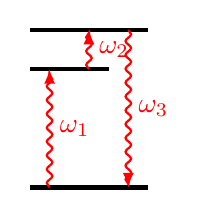
\begin{tikzpicture}[
      ph/.style={
        -latex,
        decorate,
        decoration={snake,amplitude=1,segment length=5pt},
        red,
        thick
      },
      lvl/.style={
        ultra thick
      },
      % scale=0.8,
      scale = 0.5,
      ]

      \begin{scope}
        \draw[lvl] (0,0) -- +(3,0);
        \draw[lvl] (0,3) -- +(2,0);
        \draw[lvl] (0,4) -- +(3,0);
        \draw[ph] (.5,0) -- +(0,3) node[midway,right] {$\omega_1$};
        \draw[ph] (1.5,3) -- +(0,1) node[midway,right] {$\omega_2$};

        \draw[lvl] (2,0) -- +(1,0);
        \draw[lvl] (2,4) -- +(1,0);
        \draw[ph] (2.5,4) -- +(0,-4) node[midway,right] {$\omega_3$};
      \end{scope}
    \end{tikzpicture}
    \caption{Up-conversion}
    \label{fig:up}
  \end{figure}

  \begin{figure}
    \centering
    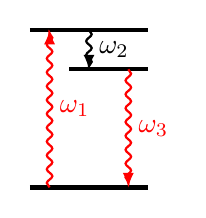
\begin{tikzpicture}
      [
      ph/.style={
        -latex,
        decorate,
        decoration={snake,amplitude=1,segment length=5pt},
        red,
        thick
      },
      noph/.style={
        -latex,
        decorate,
        decoration={snake,amplitude=1,segment length=5pt},
        black,
        thick
      },
      lvl/.style={
        ultra thick
      },
      % scale=0.8,
      scale = 0.5,
      ]
      \begin{scope}[xshift=5cm]
        \draw[lvl] (0,0) -- +(3,0);
        \draw[lvl] (0,4) -- +(3,0);
        \draw[lvl] (1,3) -- +(2,0);

        \draw[ph] (0.5,0) -- +(0,4) node[midway,right] {$\omega_1$};
        \draw[noph] (1.5,4) -- +(0,-1) node[midway,right] {$\omega_2$};
        \draw[ph] (2.5,3) -- +(0,-3) node[midway,right] {$\omega_3$};
      \end{scope}
    \end{tikzpicture}
    \caption{Down-conversion}
    \label{fig:down}
  \end{figure}

\end{columns}

  
  % \end{center}
\end{frame}



\begin{frame}{Applications}
  \begin{figure}
    \centering
    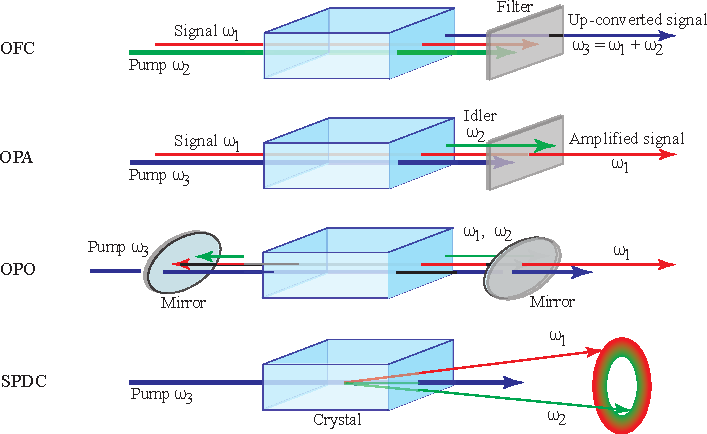
\includegraphics[width=\columnwidth]{applications}
    \caption{Applications}
    \label{fig:applications}
  \end{figure}

\end{frame}

\begin{frame}{Numerical setup}
  \begin{itemize}
  \item For up-conversion, $\omega_{3} = \omega_{1} + \omega_{2}$.
  \item RWA and SVEA.
\end{itemize}

\begin{align*}
\paren{ \pdiff{}{z}  + \frac{1}{v_i^{g}} } \mathcal{E}_i \paren{z, t}
&= \frac{i 2 \pi \omega_i^{2}}{k c^2} \mathbf{P}^{NL} \paren{z,t} e^{i \paren{k_i z - \omega_{i}
    t}} \Rightarrow \\%\tag{[Shen, equation 3.39]}\\
% \paren{ \pdiff{}{z}  + \frac{1}{v_i^{g}} } \mathcal{E}_i \paren{z, t}
% &= \frac{i \omega_i \chi^{(2)}}{2 n_i c} \mathcal{E}_j^{*}\mathcal{E}_k e^{i (k_k - k_j -k_i) z}, \text{where } i \neq j \neq k \\
\paren{ \pdiff{}{z}  + \frac{1}{v_1^{g}} } \mathcal{E}_1 \paren{z, t}
&= \frac{i \omega_1 \chi^{(2)}}{2 n_1 c} \mathcal{E}_2^{*}\mathcal{E}_3 e^{i (k_3 - k_2 -k_1) z
t} \\
\paren{ \pdiff{}{z}  + \frac{1}{v_2^{g}} } \mathcal{E}_2 \paren{z, t}
&= \frac{i \omega_2 \chi^{(2)}}{2 n_2 c} \mathcal{E}_1^{*}\mathcal{E}_3 e^{i (k_3 - k_1 -k_2) z
t} \\
\paren{ \pdiff{}{z}  + \frac{1}{v_3^{g}} } \mathcal{E}_3 \paren{z, t}
&= \frac{i \omega_3 \chi^{(2)}}{2 n_3 c} \mathcal{E}_1\mathcal{E}_2 e^{-i (k_1 - k_2 -k_3) z
t}, \\
\end{align*}

\begin{itemize}
\item Crank-Nicolson solution.
\item Alternative: Iterative Runge-Kutta for discrete points in time.
\end{itemize}


\end{frame}
 



\begin{frame}{Higher orders}
  \begin{itemize} 
  \item Third order $\Rightarrow$ Four-wave mixing in centrosymmetric materials: Example of up to $93.7\%$ efficiency.
  \item etc.
  \end{itemize}

\end{frame}



%%% Local Variables: 
%%% mode: latex
%%% TeX-master: "nonlinearslides"
%%% TeX-engine: default
%%% End: 
